\section{Problem Overview}
One of the things currently unclear with respect to this piece of research is the
specification of the problems, and how we are sending that information to an LLM.
There are two things we think we'll want to do:

\paragraph*{Synthesizing numerical/structural expressions related to data:}
\begin{figure}
      \begin{subfigure}{0.4\textwidth}
         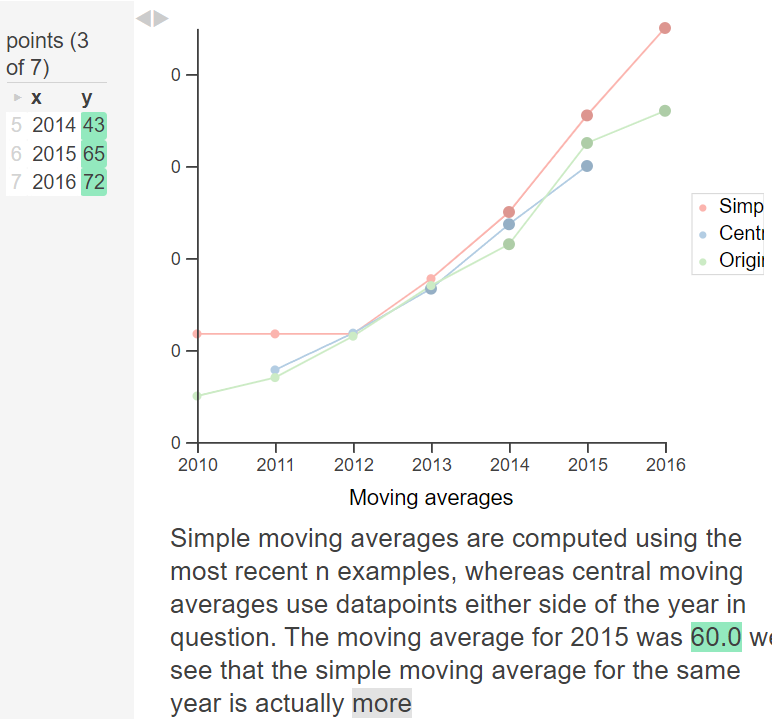
\includegraphics[width=\textwidth]{fig/text-viz.png}
         \caption{Example of text linking, using moving average example program}
         \label{fig:mavg}
      \end{subfigure}
      \hfill
      \begin{subfigure}{0.5\textwidth}
         \begin{subfigure}{\textwidth}
            \tiny
            \begin{lstlisting}[language=Fluid]
               ~\dots~
               "explain-1" :=
                  LinkedText( [ ~\dots~
                              , numToStr (getByX 2015 cavgs).y, " "
                              ~\dots~ ] )
               ~\dots~
            \end{lstlisting}
            \caption{Accessing data from chart points}
            \label{fig:synthex-1}
         \end{subfigure}
         \vfill
         \begin{subfigure}{\textwidth}
            \tiny
            \begin{lstlisting}[language=Fluid]
               ~\dots~
               let leqP n m = 
                  if n <= m
                  then "less"
                  else "more";
               ~\dots~
               , leqP (getByX 2015 savgs).y (getByX 2015 cavgs).y
               ~\dots~
            \end{lstlisting}
            \caption{generating text from results of data comparisons}
            \label{fig:synthex-2}
         \end{subfigure}
      \end{subfigure}
   \caption{Small Synthesis Examples}
   \label{fig:synthex}
\end{figure}
if we are referring to a simple aggregate summary of data, we want to be able
to synthesize an in-place expression that helps out explanation. For example,
if we are explaining a bar-chart, we might write code that looks like \figref{synthex-1}.
In many cases, we can write this ourselves, but would like to be able to
synthesize the highlighted expression.

\paragraph*{Synthesizing string expressions based on those numerical expressions:}
this is similar to the nombre library in R, once we are able to synthesize references
to numerical expressions and data, we want to be able to take those, and use them to
create small strings to splice into an explanation. For example, in \figref{synthex-2}
we would like the tool to be able to synthesize both the function \kw{leqP}, and
the expression in situ, which then generates the last word in the caption appearing in
\figref{mavg}.
